\documentclass[]{../common/elementary-physics}

\title{5. Increasing Electromagnet Force}
\date{2015-11-19 v0.6}

\begin{document}

\maketitle

\tableofcontents

\section{Abstract}

Since the concept of an electromagnet is present in both motors and generators we find it interesting to study the relationship between the parameters describing the electrical power the coil draws and the mechanical force with which the coil attracts a piece of ferromagnetic material or a magnet.

\section{Clues}

Go to any site with detailed information on electromagnets of various sizes, like Highcap\cite{highcap}, and collect the data, normalize it and calculate $F/P$:

\begin{center}
\begin{tabular}{r|r|r|r|r|r|r}
\head{d $mm$} & \head{h $mm$} & \head{F $N$} & \head{P $W$} & \head{F/P} & \head{A $mm^2$} & \head{F/PA} \\
\hline
20 &	15 &	20 &	3 &	6.5 &	300 &	0.022 \\
25 &	20 &	49 &	4 &	12.3 &	500 &	0.025 \\
30 &	22 &	98 &	4 &	24.5 &	660 &	0.037 \\
34 &	18 &	177 &	4 &	44.1 &	612 &	0.072 \\
40 &	20 &	196 &	8 &	24.5 &	800 &	0.031 \\
49 &	21 &	392 &	10 &	39.2 &	1029 &	0.038 \\
60 &	34 &	686 &	13 &	52.8 &	2040 &	0.026 \\
65 &	30 &	785 &	13 &	60.3 &	1950 &	0.031
\end{tabular}
\end{center}

As you can see we have also calculated $A$ as a kind of cross-section area $A=d \, h$ and $F/PA$ which seems as if it could be a constant.
We plot $F/P$ as a function of $A$:

\begin{figure}[ht] \centering
	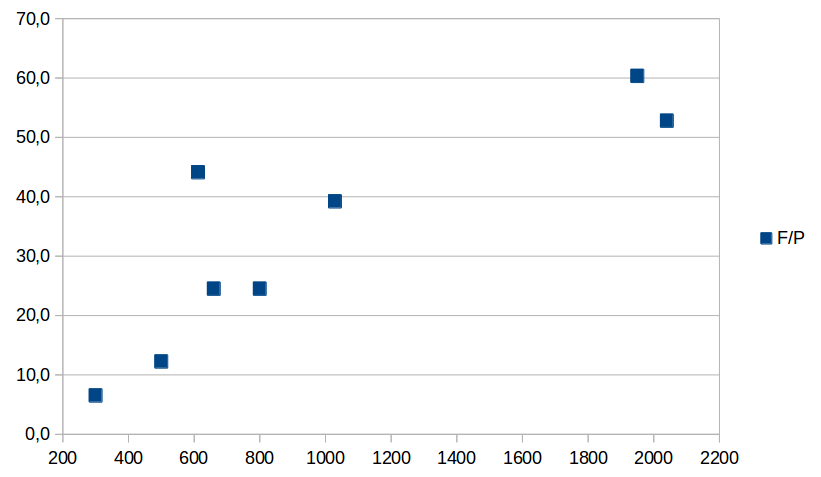
\includegraphics[scale=.4]{fp-of-a-2} \caption{F/P(A)}
\end{figure}

The only outstanding data-point in this collection seems to be the fourth electromagnet.

The same investigation can be done on PMDC motors.
Plot the torque times speed to input power ratio as a function to its size and you will see that bigger motors give higher values.

\section{Formula}

Searching for a formula on this relationship we found\cite{wpele,gbet}:

\begin{equation}
F = \frac{\mu^2}{2 \, \mu_0 \, g^2} \, N^2 \, I^2 \, A
\end{equation}

where $g$ is the air-gap.
Let us introduce $A_F$ to make it easier to read:

\begin{equation}
A_F = \frac{\mu^2 A}{2 \, \mu_0 \, g^2}
\end{equation}

and we get:

\begin{equation}
F = A_F \, N^2 \, I^2
\end{equation}

Let us introduce a new concept; the relationship between the resistance and the number of turns in an inductor:

\begin{equation}
R = A_R \, N^2
\end{equation}

$A_R$ is the form-factor of the windings of the inductor.
Roughly we have:

\begin{equation}
A_R = 11 \rho \, \frac{r}{d \, l}
\end{equation}

where $\rho$ is the resistivity of the material in the wire, which for copper is $16.78 \si{\nano\ohm\metre}$, $r$ is mean radius, $d$ is depth and $l$ is length.

The definition of $A_R$ makes it possible to rewrite the formula:

\begin{subequations}
\begin{align}
F &= A_F \, \frac{R}{A_R} \, I^2 \\
F &= A_F \, \frac{P}{A_R} \\
\frac{F}{P} &= \frac{A_F}{A_R}
\end{align}
\end{subequations}

It seems that the $F/P$ ratio for an electromagnet is not a function of the number of turns, but apart from core-related parameters rather the amount of copper-wire; the more wire-mass, the bigger the form, the smaller the $A_R$ the stronger force per input-power.

We can also say that for any electromagnet, the force is proportional to the power, when we increase the power the force increase:

\begin{equation}
F = \frac{A_F}{A_R} P
\end{equation}

\pagebreak

\section{Experiment}

Eight coils a-h have been tested, five on a small form and three on a big form.
They all had welding rods as their cores.

\begin{figure}[ht] \centering
	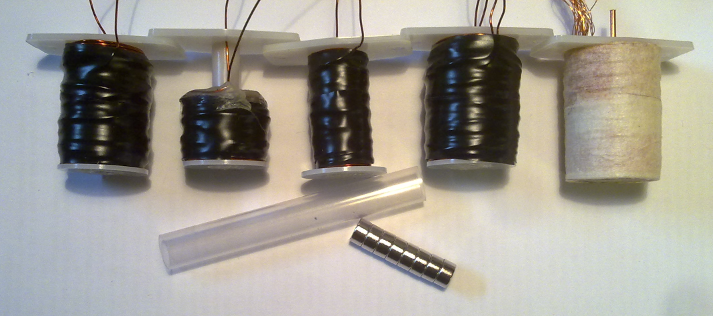
\includegraphics[scale=1.7]{coils-a-e} \caption{Coils a-e}
\end{figure}

\begin{figure}[ht] \centering
	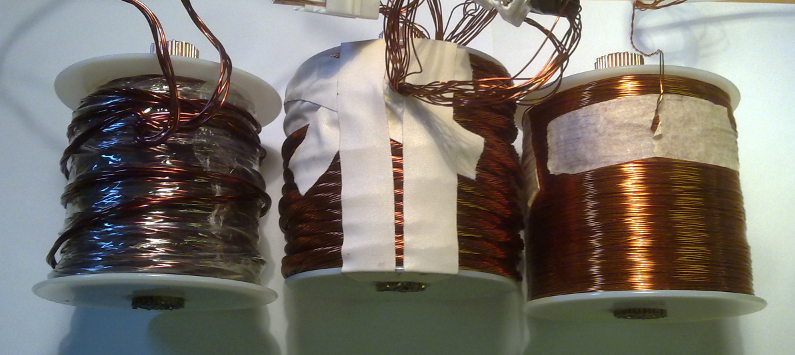
\includegraphics[scale=1.7]{coils-f-h} \caption{Coils f-h}
\end{figure}

The testing was conducted using a small plastic tube and a stack of small magnets that could easily slide in the tube.
The coil to be tested was placed on a table with its core in a vertical position, the tube with the magnets was placed on top of the core so the magnets would be lifted once the current started to flow.
Voltage and current were measured when the magnets were lifted to the same height as for coil c.
The current chosen for coil c was related to the limits of the power-supply.
Both voltage and current were measured with meters external to the power-supply.

\begin{landscape}

\tiny
\begin{tabular}{	r	|	l	|	r	|	r	|	r	|	r	|	r	|	r	|	r	|	r	|	r	|	r	|	r	|	r	|	r	|	r	|	r	|	r	|	r	|	r	|	r	}
\head{	coil	} & \head{	comment	} & \head{	$r$	} & \head{	$d$	} & \head{	$l$	} & \head{	$\varrho$ } & \head{	$A_R$	} & \head{	$A$	} & \head{	$m_{tot}$	} & \head{	$m_{Cu}$	} & \head{	$W_d$	} & \head{	$N$	} & \head{	$R$	} & \head{	$A_R$	} & \head{	$L$	} & \head{	$A_L$	} & \head{	$V$	} & \head{	$I$	} & \head{	$P$	} & \head{	$N^2 I^2 A$	} & \head{	$P m$	} \\
\hline																																										
		&	air core, no wire	&	8.4	&	8.7	&	34.5	&	1	&	5.2	&		&	4.2	&		&		&		&		&		&		&		&		&		&		&		&		\\
		&	welding rods core, no wire	&	8.4	&	8.7	&	34.5	&	1	&	5.2	&	30	&	11.0	&		&		&		&		&		&		&		&		&		&		&		&		\\
	a	&	1 x 1, full	&	8.4	&	8.7	&	34.5	&	1	&	5.2	&	30	&	94.4	&	83.4	&	0.6	&	693	&	2.4	&	5.1	&	8.13	&	16.93	&	3.8	&	1.4	&	5.35	&	29.4	&	446	\\
	b	&	1 x 1, half length	&	8.4	&	8.7	&	17.3	&	1	&	10.4	&	30	&	54.9	&	43.8	&	0.6	&	350	&	1.2	&	10.1	&	2.57	&	20.98	&	3.3	&	2.1	&	7.01	&	16.5	&	307	\\
	c	&	1 x 1, half depth	&	6.2	&	4.3	&	34.5	&	1	&	7.7	&	30	&	44.3	&	33.3	&	0.6	&	350	&	1.0	&	8.5	&	2.04	&	16.65	&	4.0	&	2.9	&	11.67	&	31.8	&	388	\\
	d	&	1 x 2, (in series)	&	8.4	&	8.7	&	34.5	&	1	&	5.2	&	30	&	99.7	&	88.6	&	0.6	&	700	&	2.5	&	5.2	&	8.25	&	16.84	&	3.9	&	1.4	&	5.50	&	29.4	&	487	\\
	d	&	1 x 1, (half wires)	&	8.4	&	8.7	&	34.5	&	0.5	&	10.4	&	30	&	99.7	&	44.3	&	0.6	&	350	&	1.3	&	10.4	&	2.06	&	16.82	&	4.3	&	2.8	&	11.84	&	28.2	&	525	\\
	d	&	2 x 1, (in parallel)	&	8.4	&	8.7	&	34.5	&	1	&	5.2	&	30	&	99.7	&	88.6	&	0.6	&	350	&	0.7	&	6.0	&	2.07	&	16.90	&	2.6	&	2.8	&	7.49	&	29.9	&	664	\\
	e	&	1 x 1, full	&	8.4	&	8.7	&	34.5	&	1	&	5.2	&	30	&	107.3	&	96.3	&	0.2	&	6000	&	177.0	&	4.9	&	672.00	&	18.67	&	26.3	&	0.1	&	3.89	&	23.8	&	375	\\
		&	air core, no wire	&	28.7	&	32.5	&	77.6	&	1	&	2.1	&		&	39	&		&		&		&		&		&		&		&		&		&		&		&		\\
		&	welding rods core, no wire	&	28.7	&	32.5	&	77.6	&	1	&	2.1	&	302	&	241	&		&		&		&		&		&		&		&		&		&		&		&		\\
	f	&	4 x 1, not full	&	24.5	&	24.4	&	77.6	&	1	&	2.4	&	302	&	1438	&	1197	&	1	&	300	&	0.3	&	2.8	&	4.07	&	45.22	&	0.8	&	1.7	&	1.38	&	78.7	&	1650	\\
	g	&	5 x (3*2), overfull	&	29.2	&	33.7	&	77.6	&	1	&	2.1	&	302	&	2576	&	2335	&	0.6	&	1224	&	2.7	&	1.8	&	68.89	&	45.98	&	1.2	&	0.4	&	0.50	&	77.1	&	1171	\\
	g	&	5 x 3, overfull	&	29.2	&	33.7	&	77.6	&	0.5	&	4.1	&	302	&	2576	&	1168	&	0.6	&	612	&	1.5	&	4.1	&	17.14	&	45.77	&	1.2	&	0.8	&	0.98	&	70.3	&	1141	\\
	g	&	(2*5) x 3, overfull	&	29.2	&	33.7	&	77.6	&	1	&	2.1	&	302	&	2576	&	2335	&	0.6	&	612	&	0.7	&	2.0	&	17.15	&	45.79	&	0.8	&	0.8	&	0.62	&	74.3	&	1458	\\
	h	&	1 x 1, almost full	&	26.7	&	28.4	&	77.6	&	1	&	2.2	&	302	&	2322	&	2081	&	0.5	&	7200	&	92.6	&	1.8	&	2760.00	&	53.24	&	7.1	&	0.1	&	0.52	&	83.4	&	1082	\\
\end{tabular} 																	
																								\\
\\
\\

\begin{tabular}{	l	|	l	|	l	}
\head{header} & \head{unit} & \head{definition} \\
\hline																				coil		&				& label	\\
comment		&				& p x s number of strands in parallel times number of strands in series	\\
$r$			& $mm$			& mean radius for the windings \\
$d$			& $mm$			& depth for the windings \\
$l$			& $mm$			& core-length \\
$\varrho$	&				& windings density, how much used, times $8/11$ \\
$A_R$		& $\mu \ohm$	& calculated from dimensions using formula \\
$A$			& $mm^2$		& core area \\
$m_{tot}$	& $g$			& mass \\
$m_{Cu}$	& $g$			& copper mass \\
$W_d$		& $mm$			& wire diameter \\
$N$			&				& number of turns \\
$R$			& $\ohm$		& resistance \\
$A_R$		& $\mu \ohm$	& calculated from resistance \\
$L$			& $mH$			& inductance \\
$A_L$		& $nH$			& calculated from inductance \\
$V$			& $V$			& voltage applied \\
$I$			& $A$			& current drawn \\
$P$			& $W$			& power drawn \\
$N^2 I^2 A$	& $A^2 mm^2$	& part of the original expression for F \\
$P m$		& $W g$			& power times mass \\
\end{tabular}

\end{landscape}

The pole-area of the magnets was $50 mm^2$, very well suited for coils a-e, but coil f-h has a much greater core-area than the magnets which makes comparisons between the two sets of coils difficult.

One surprise was the power drawn by coil f which we will have to look deeper into.

Watch a short, hasty and inexact version of the experiment with coil a,b and e at \url{https://www.youtube.com/watch?v=IIeRR6NjMPQ}.



\section{Conclusion}

Although more can be explored in this area the general rule to get the best performance out of an electromagnet is to have the electromagnet as big as possible, which leads us to believe that motors should have as few and big coils as possible\cite{jonew} to increase torque per power.
We also believe that the reverse is true, that generators should have as many and small coils as possible to decrease torque per power.

\appendix

\section{In Plain English}

Whenever we spend something, be it time, money, energy or power, we want to get the most value back, so we calculate the performance per input ratio.
In this paper we have proposed a way of doing the same with electromagnets.
The amount of copper in an electromagnet is one important factor that affects the force per power ratio, not the number of turns or the wire thickness in the coil.
The general rule is; the more copper the greater force.

\section{På Ren Svenska}

När vi spenderar något, vare sig det är tid, pengar, energi eller kraft, vi vill få ut mesta möjliga tillbaka, så vi beräknar förhållandet mellan prestanda och input.
I den här artikeln har vi föreslagit ett sätt att göra samma sak med elektromagneter.
Mängden koppar i en elektromagnet är en viktig faktor som påverkar förhållandet mellan kraft och effekt, inte antalet varv eller trådtjocklek i spolen.
Den generella regeln är; ju mer koppar desto större kraft.

\section{$A_F$, $A_R$ and $A_L$}

$A_F$ was introduced to bundle the core-related parameters together.

$A_R$ is the form-factor of the windings of the inductor.
If $W$ is the wire then we have:

\begin{subequations}
\begin{align}
R &= \rho \frac{W_{length}}{W_{area}} \\
N &= \frac{d}{W_{diam}} \, \frac{l}{W_{diam}} \\
W_{length} &= 2 \pi r \, N \\
W_{area} &= \frac{\pi}{4} \frac{d \, l}{N} \\
R &= \frac{\rho}{\varrho} \frac{2 \pi r \, N \, 4 N}{\pi \, d \, l} \\
R &= 8 \frac{\rho}{\varrho} \frac{r}{d \, l} N^2 \\
A_R &= 8 \frac{\rho}{\varrho} \frac{r}{d \, l} \\
R &= A_R N^2
\end{align}
\end{subequations}

where $\rho$ is the resistivity of the material in the wire, which for copper is $16.78 \si{\nano\ohm\metre}$, $\varrho$ is the tightness of the windings, $r$ is the mean radius, $d$ is the depth and $l$ is the length.
A realistic value for $\varrho$ seems to be $8/11$ which gives us:

\begin{equation}
A_R = 11 \rho \frac{r}{d \, l}
\end{equation}

which is what we use.
$A_R$ is similar in its definition to $A_L$.

$A_L$ is frequently specified by transformer-core manufacturers.
The definition is and can for a multilayer air-core coil be calculated as\cite{wpind}: 

\begin{subequations}
\begin{align}
L &= A_L \, N^2 \\
A_L &= \frac{4}{5} \frac{r^2}{6r+9l+10d}
\end{align}
\end{subequations}

The time-constant for a coil can now be expressed as:

\begin{equation}
\tau_L = \frac{L}{R} = \frac{A_L N^2}{A_R N^2} = \frac{A_L}{A_R}
\end{equation}

and is therefore constant for a given core and form regardless of the choice of wire gauge as long as the form is equally filled with wire.

\section{This Paper}

This is one paper from a collection of papers, all free to be downloaded and shared. If you have ideas how to enhance any of the papers, if you want to contribute, don’t hesitate to contact us at \url{hob.nilre@gmail.com}.\\
\\
The papers can all be found at:
\begin{itemize}
\item \url{https://sites.google.com/site/nilrehob/home/elementary-physics}
\item \url{https://independent.academia.edu/HobNilre/Papers}
\item \url{https://groups.yahoo.com/neo/groups/EVGRAY/files/Hob/}
\item \url{http://overunity.com/15796/elementary-physics-revisited/}
\item \url{http://idipsum.se/home/elementary%20physics.html}
\item \url{https://github.com/boherlin/elementary-physics/tree/master/pdf}
\end{itemize}

They are updated with new versions in an unpredictable manner, possibly not on all sites but at least on the last two sites in the list, make sure you always have the latest version!
Their \LaTeX source-codes can be found at \url{https://github.com/boherlin/elementary-physics/tree/master/src}.
All papers, but not all versions, have been stamped at \url{http://www.OriginStamp.org}.\\
\\
If you enjoyed this paper, found value in it and want to help us, please consider giving us a donation in bitcoin, this is our address:

\begin{figure}[ht] \centering
	
\includegraphics[]{1B79p75vQw4Rb1GQdmGYpDapFwEytFJDqw} \caption{1B79p75vQw4Rb1GQdmGYpDapFwEytFJDqw}
\end{figure}


\printbibliography

\end{document}

